\documentclass[beamer]{standalone}

\begin{document}
	\begin{frame}
		\color{blue}\centering\Huge{\textbf{Velocità}}	
	\end{frame}
	
	\begin{frame}{{Velocità}}
		\centering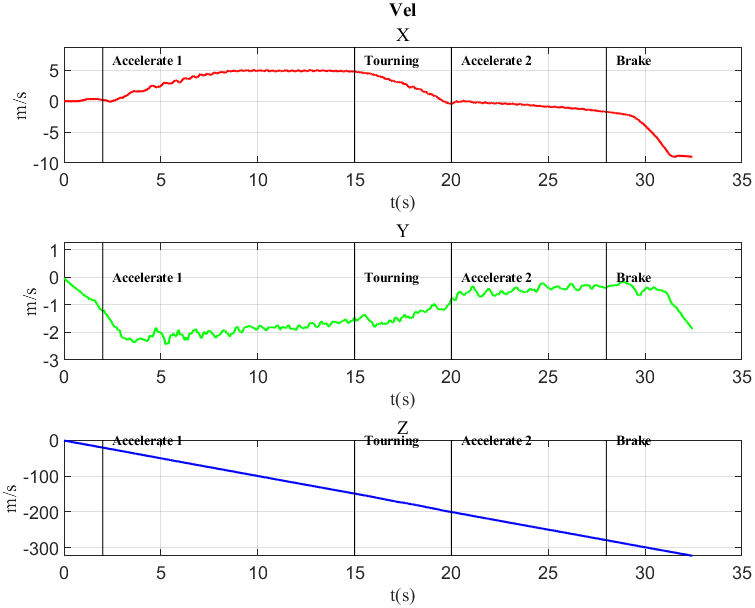
\includegraphics[height=.8\textheight]{figure/Vel/Vel}
	\end{frame}
	
%	\begin{frame}{{Media}}
%		\centering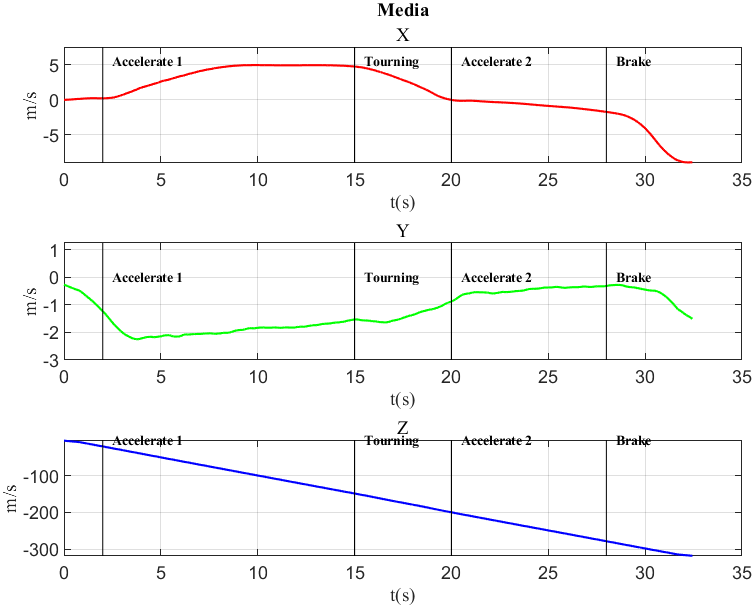
\includegraphics[height=.8\textheight]{figure/Vel/Media}
%	\end{frame}
%	
%	\begin{frame}{{Media Rettificata}}
%		\centering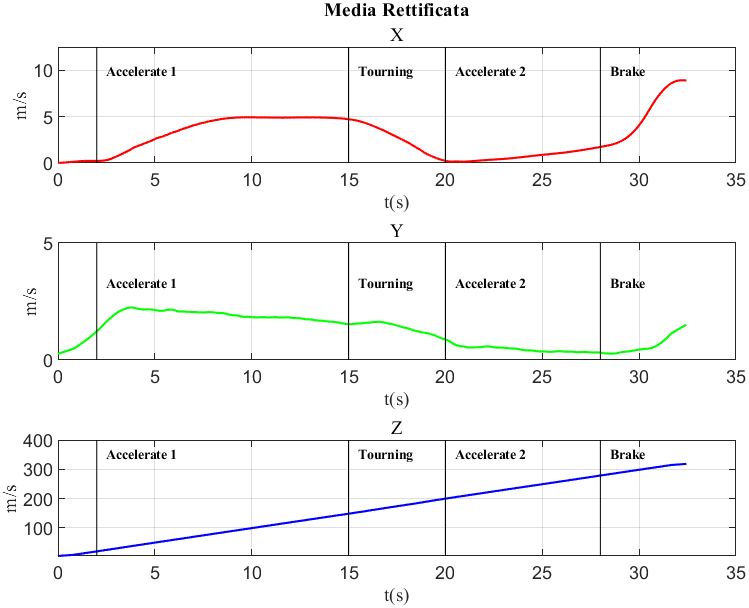
\includegraphics[height=.8\textheight]{figure/Vel/Media Rettificata}
%	\end{frame}
	
	\begin{frame}{{Varianza}}
		\centering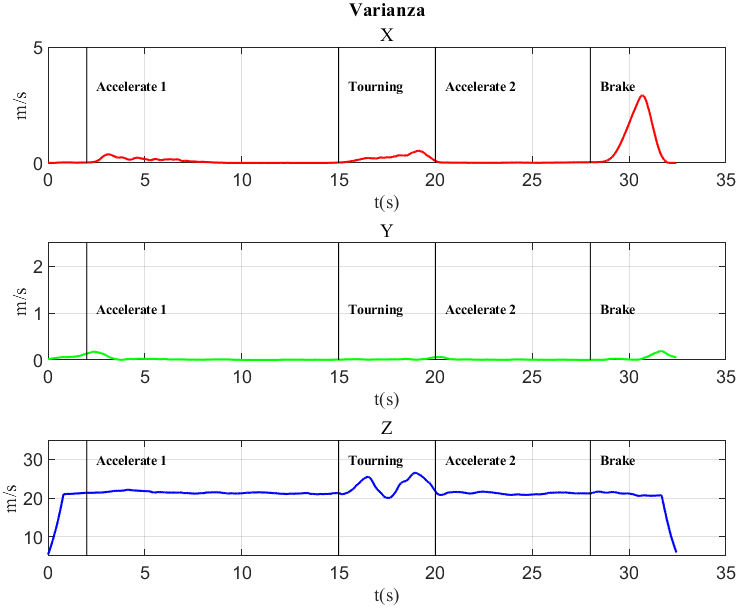
\includegraphics[height=.8\textheight]{figure/Vel/Varianza}
	\end{frame}
	
%	\begin{frame}{{Deviazione Standard}}
%		\centering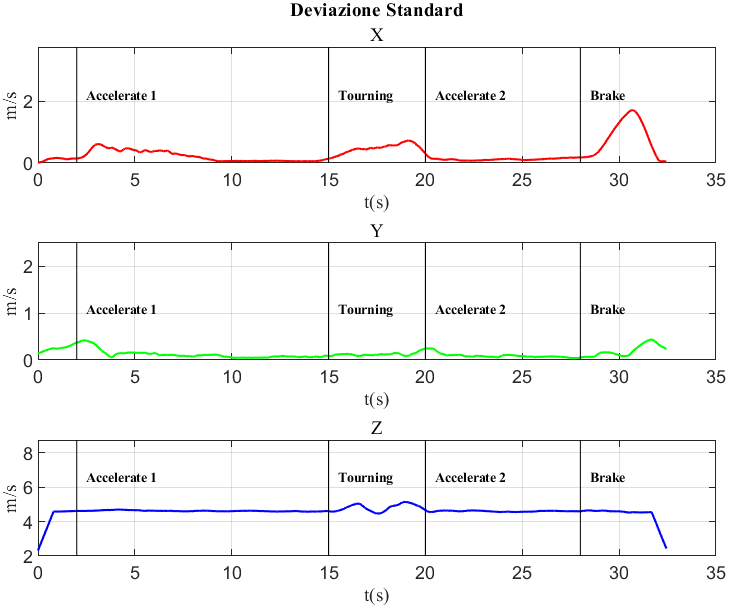
\includegraphics[height=.8\textheight]{figure/Vel/Deviazione Standard}
%	\end{frame}
	
	\begin{frame}{{Scarto Quadratico Medio}}
		\centering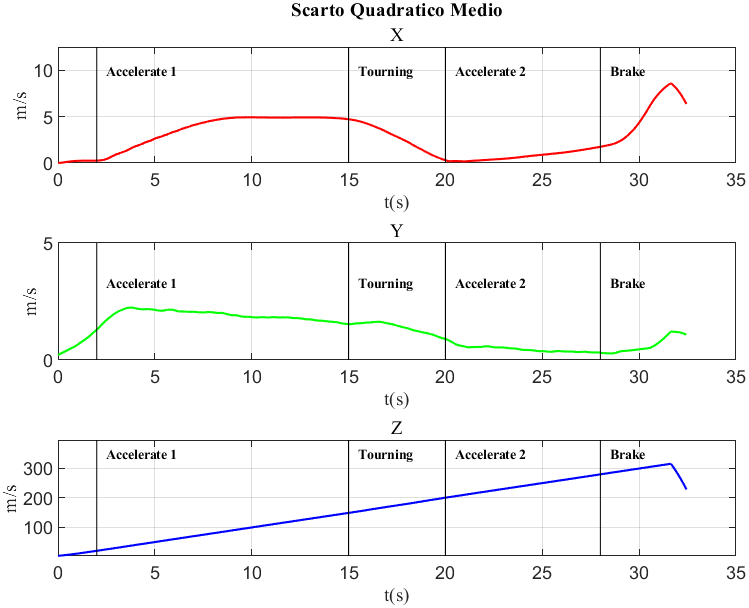
\includegraphics[height=.8\textheight]{figure/Vel/Scarto Quadratico Medio}
	\end{frame}
	
%	\begin{frame}{{Max}}
%		\centering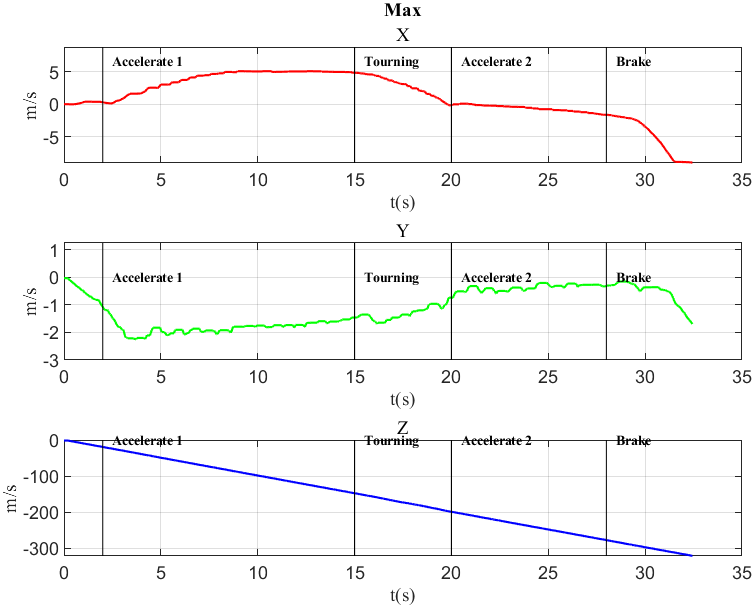
\includegraphics[height=.8\textheight]{figure/Vel/Max}
%	\end{frame}
%	
%	\begin{frame}{{Min}}
%		\centering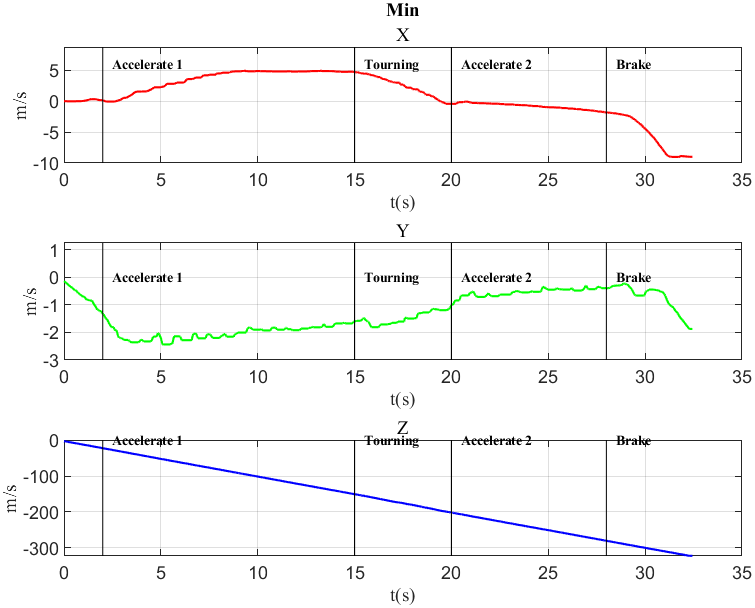
\includegraphics[height=.8\textheight]{figure/Vel/Min}
%	\end{frame}
	
	\begin{frame}{{Peak}}
		\centering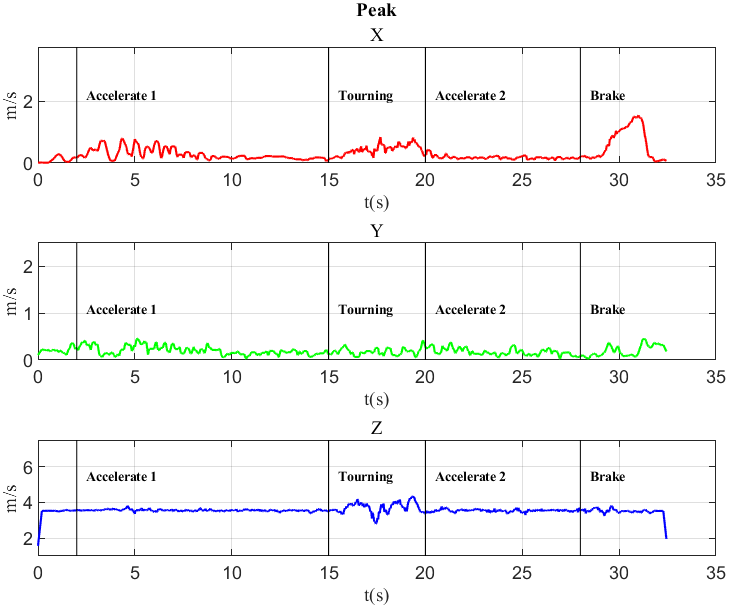
\includegraphics[height=.8\textheight]{figure/Vel/Peak}
	\end{frame}
	
%	\begin{frame}{{Kurtosi}}
%		\centering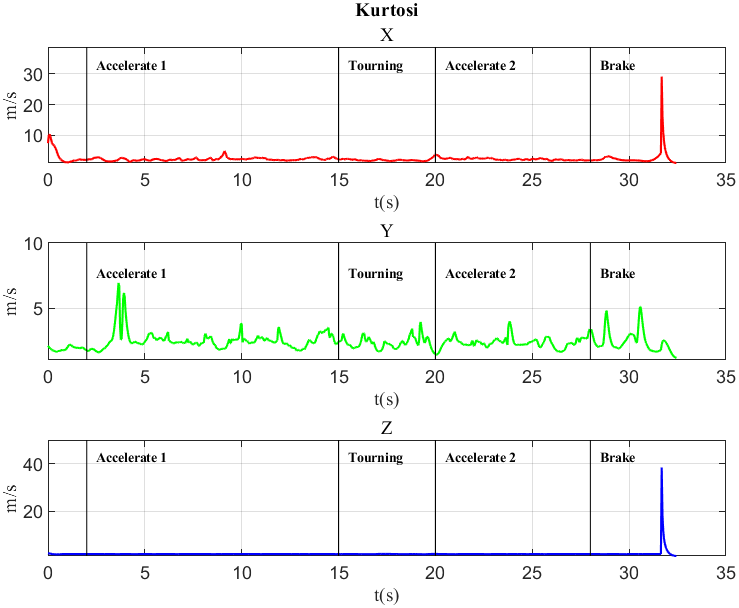
\includegraphics[height=.8\textheight]{figure/Vel/Kurtosi}
%	\end{frame}
%	
%	\begin{frame}{{Skewness}}
%		\centering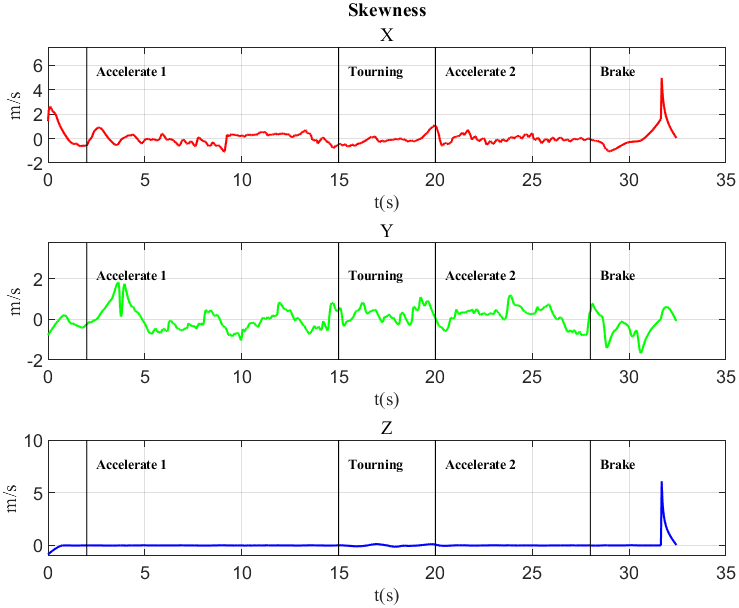
\includegraphics[height=.8\textheight]{figure/Vel/Skewness}
%	\end{frame}
	
%	\begin{frame}{{Shape Factor}}
%		\centering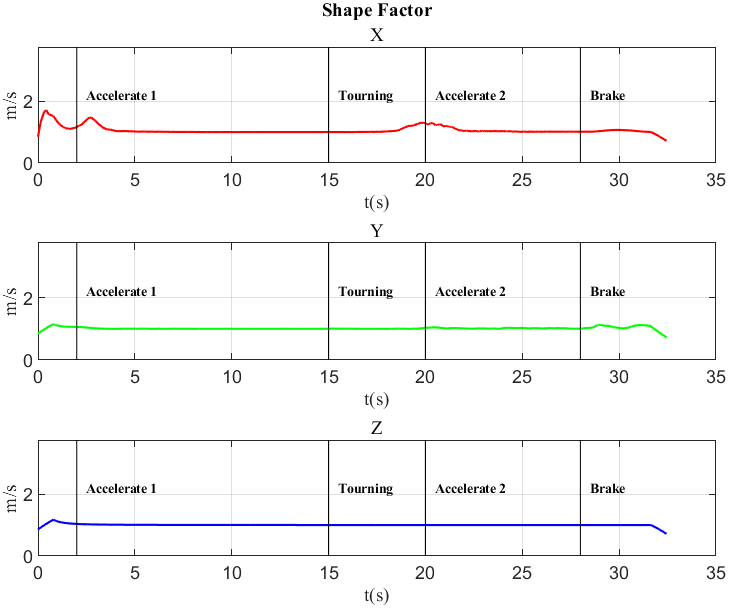
\includegraphics[height=.8\textheight]{figure/Vel/Shape Factor}
%	\end{frame}
	
	\begin{frame}{{Crest Factor}}
		\centering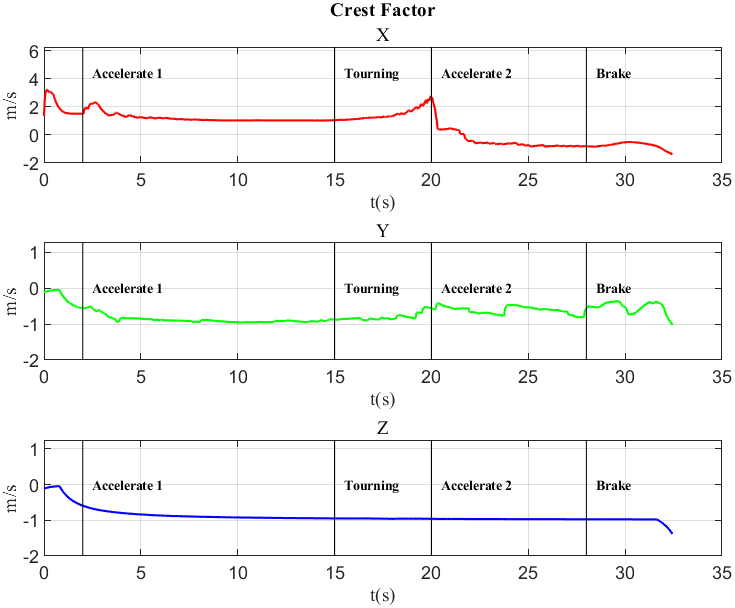
\includegraphics[height=.8\textheight]{figure/Vel/Crest Factor}
	\end{frame}
	
	\begin{frame}{{Impulse Factor}}
		\centering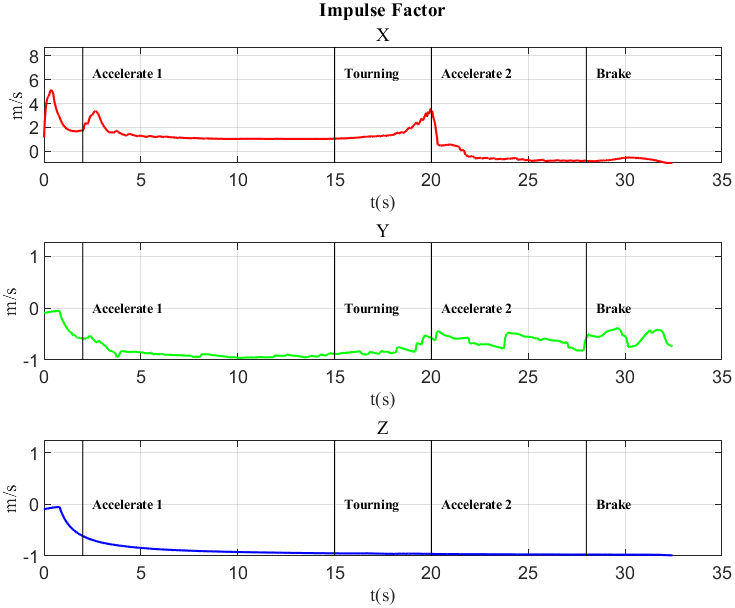
\includegraphics[height=.8\textheight]{figure/Vel/Impulse Factor}
	\end{frame}
	
	\begin{frame}{{Margin Factor}}
		\centering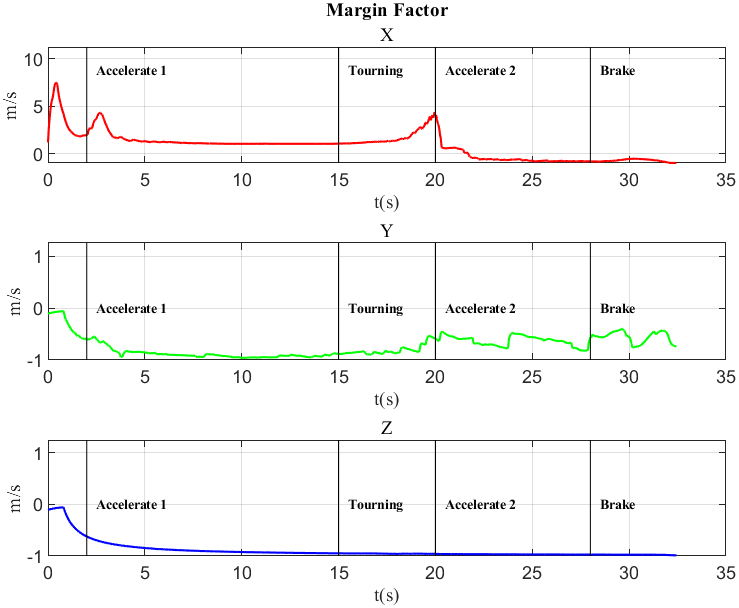
\includegraphics[height=.8\textheight]{figure/Vel/Margin Factor}
	\end{frame}
	
%	\begin{frame}{{Trasformata}}
%		\centering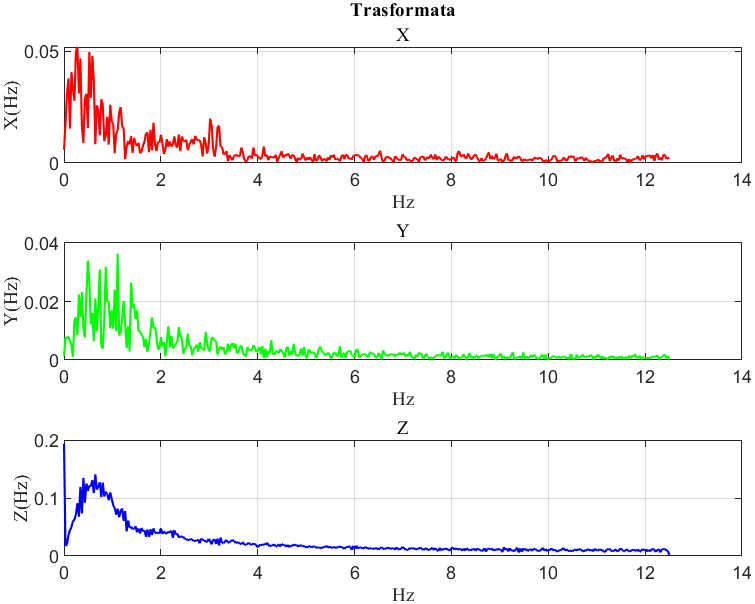
\includegraphics[height=.8\textheight]{figure/Vel/Trasformata/Trasformata}
%	\end{frame}
%	
%	\begin{frame}{{Spettro}}
%		\centering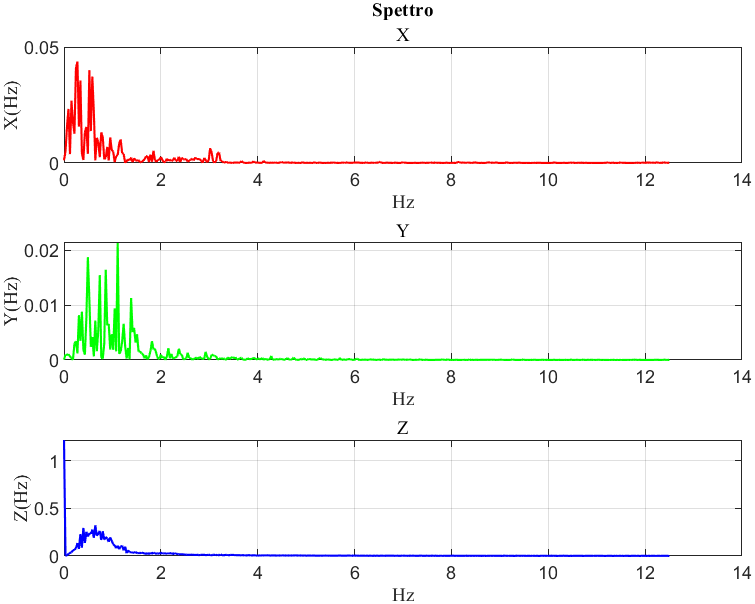
\includegraphics[height=.8\textheight]{figure/Vel/Trasformata/Spettro}
%	\end{frame}
%	
%	\begin{frame}
%		\color{blue}\centering\huge{\textbf{Trasformata Velocità}}
%	\end{frame}
%	
%	\begin{frame}{{Trasformata Accelerazione 1}}
%		\centering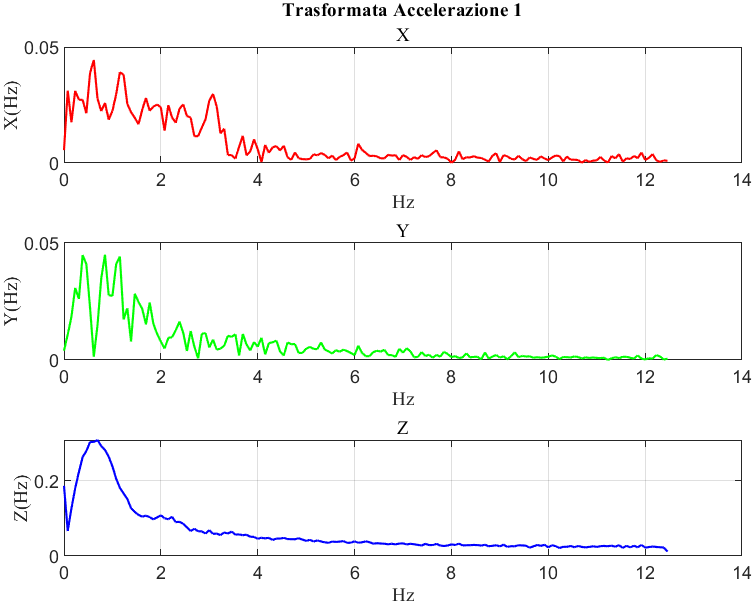
\includegraphics[height=.8\textheight]{figure/Vel/Trasformata/Trasformata Accelerazione 1}
%	\end{frame}
%	
%	\begin{frame}{{Trasformata Tourning}}
%		\centering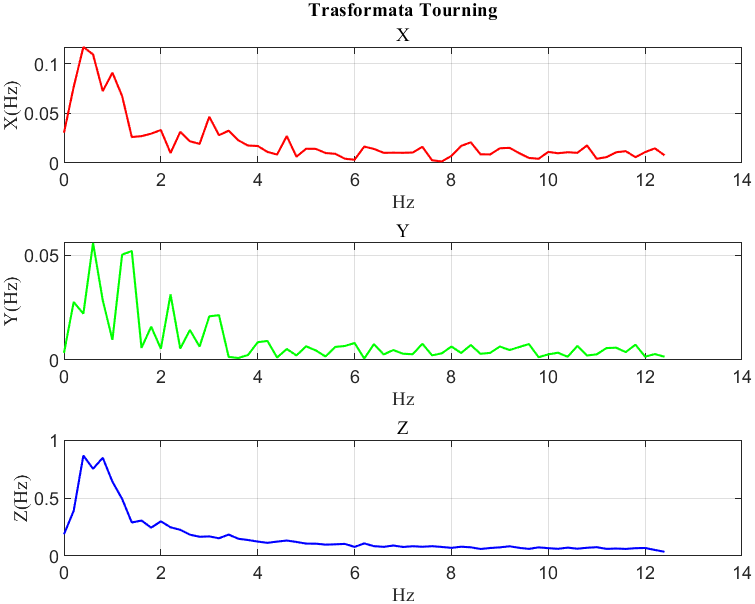
\includegraphics[height=.8\textheight]{figure/Vel/Trasformata/Trasformata Tourning}
%	\end{frame}
%	
%	\begin{frame}{{Trasformata Accelerazione 2}}
%		\centering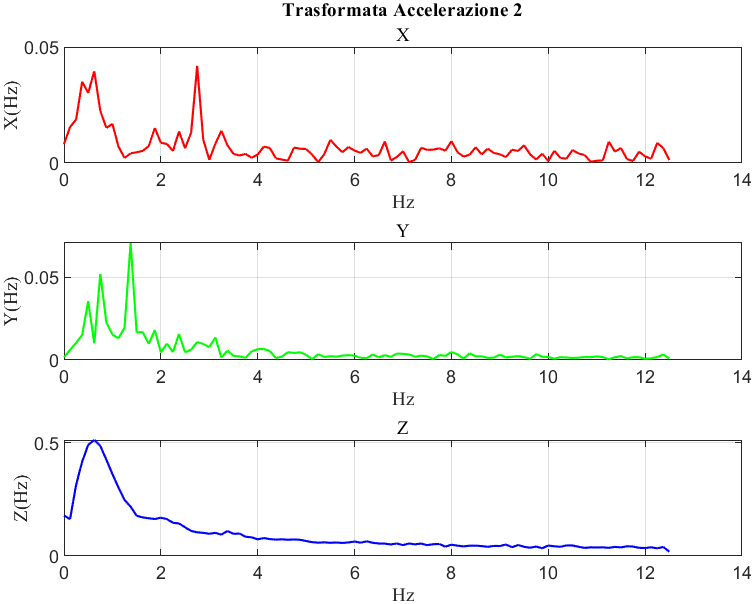
\includegraphics[height=.8\textheight]{figure/Vel/Trasformata/Trasformata Accelerazione 2}
%	\end{frame}
%	
%	\begin{frame}{{Trasformata Brake}}
%		\centering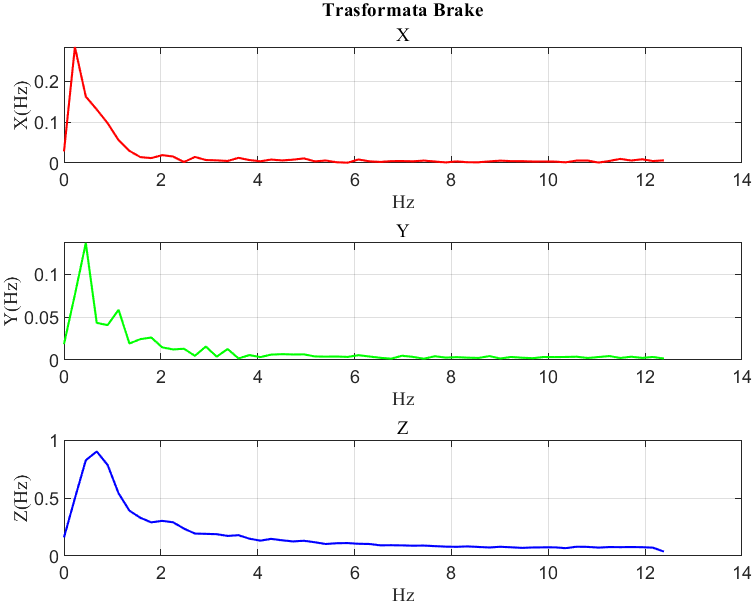
\includegraphics[height=.8\textheight]{figure/Vel/Trasformata/Trasformata Brake}
%	\end{frame}
%	
%	\begin{frame}{{Ampiezza Media X}}
%			\centering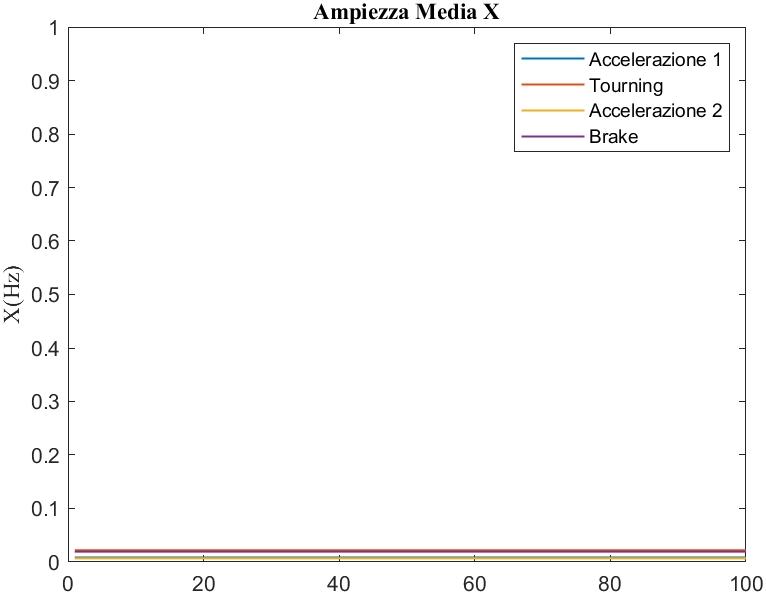
\includegraphics[height=.8\textheight]{figure/Vel/Trasformata/Ampiezza MediaX}
%	\end{frame}
%	
%	\begin{frame}{{Ampiezza Media Y}}
%		\centering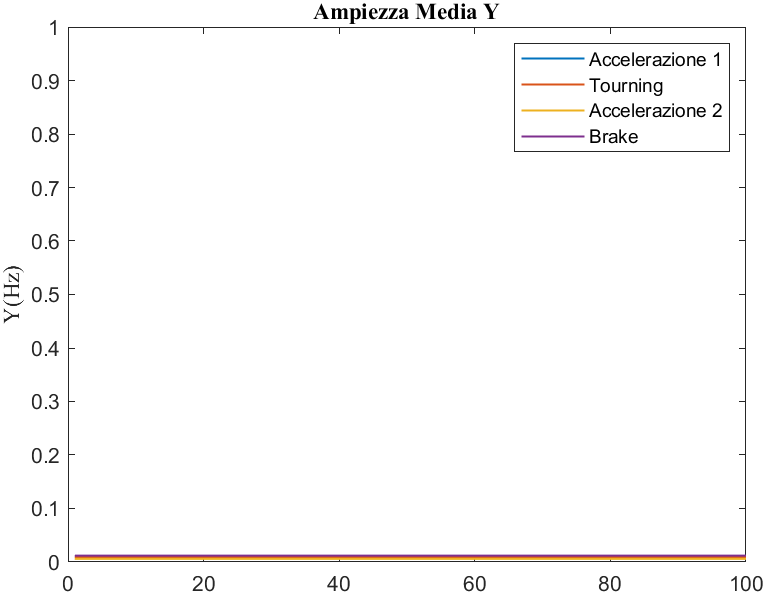
\includegraphics[height=.8\textheight]{figure/Vel/Trasformata/Ampiezza MediaY}
%	\end{frame}
%	
%	\begin{frame}{{Ampiezza Media Z}}
%		\centering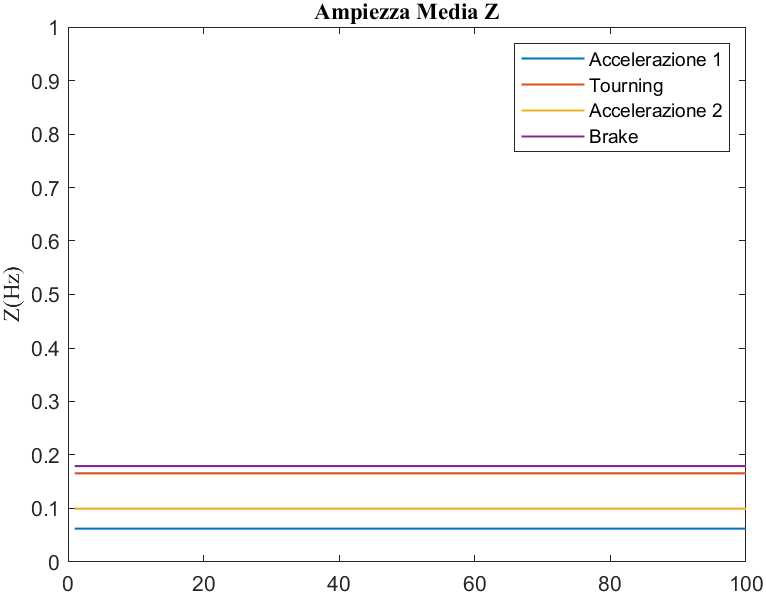
\includegraphics[height=.8\textheight]{figure/Vel/Trasformata/Ampiezza MediaZ}
%	\end{frame}
%	
%	\begin{frame}{{Frequency Centroid X}}
%		\centering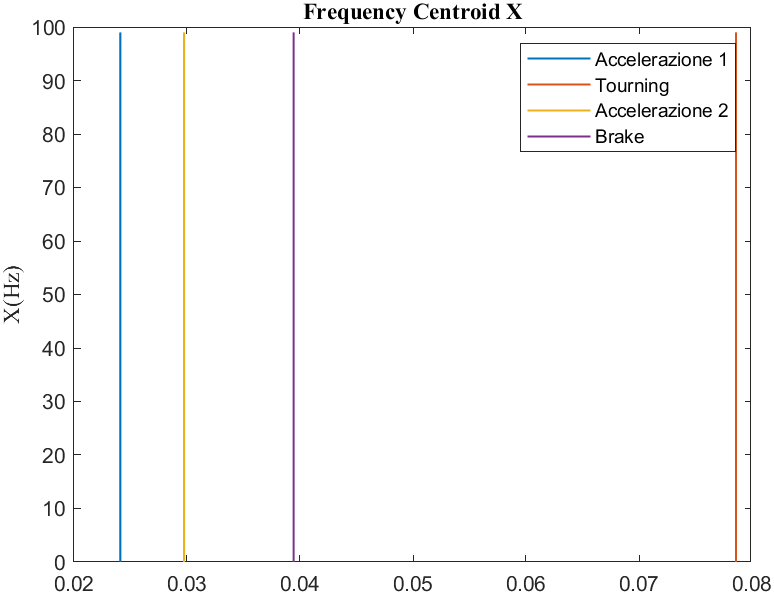
\includegraphics[height=.8\textheight]{figure/Vel/Trasformata/Frequency CentroidX}
%	\end{frame}
%
%	\begin{frame}{{Frequency Centroid Y}}
%		\centering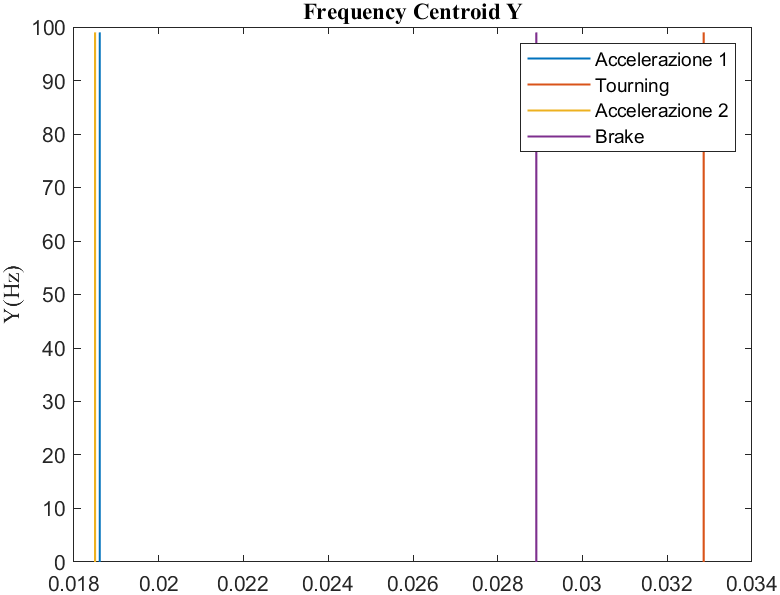
\includegraphics[height=.8\textheight]{figure/Vel/Trasformata/Frequency CentroidY}
%	\end{frame}
%	
%	\begin{frame}{{Frequency Centroid Z}}
%		\centering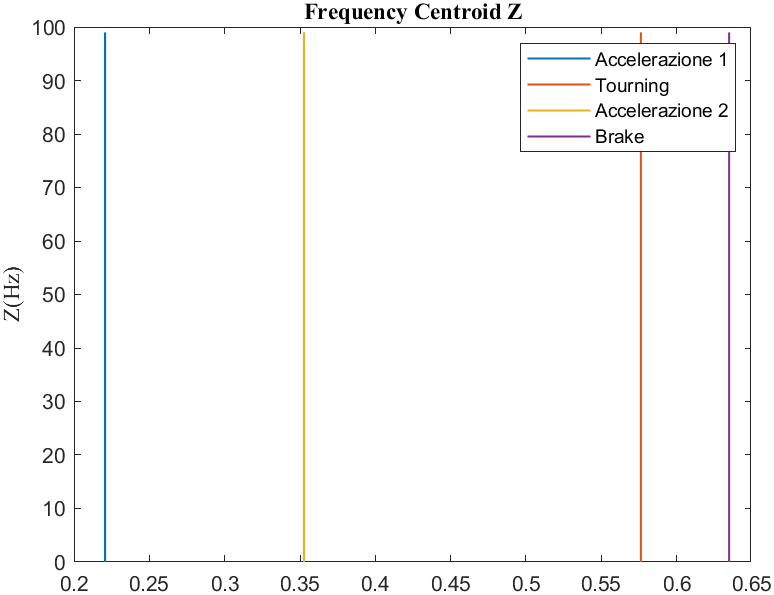
\includegraphics[height=.8\textheight]{figure/Vel/Trasformata/Frequency CentroidZ}
%	\end{frame}
%	
%	\begin{frame}{{Frequency Variance X}}
%		\centering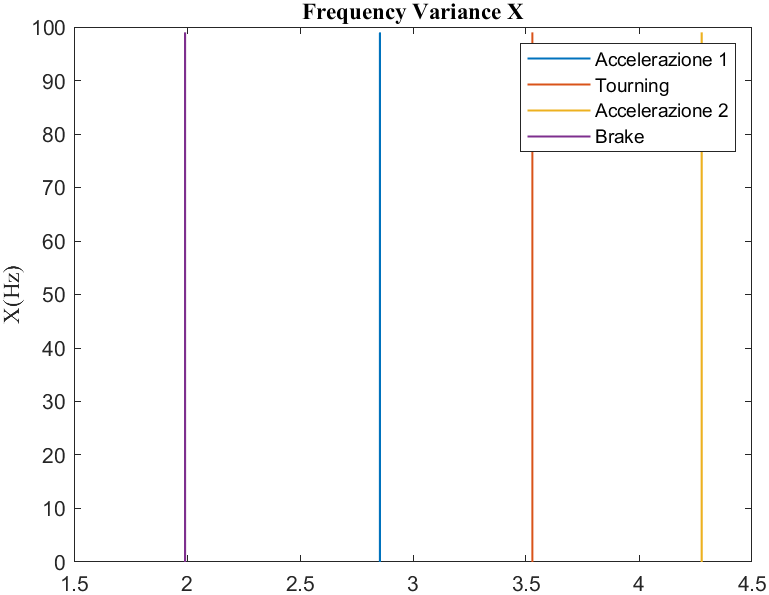
\includegraphics[height=.8\textheight]{figure/Vel/Trasformata/Frequency VarianceX}
%	\end{frame}
%	
%	\begin{frame}{{Frequency Variance Y}}
%		\centering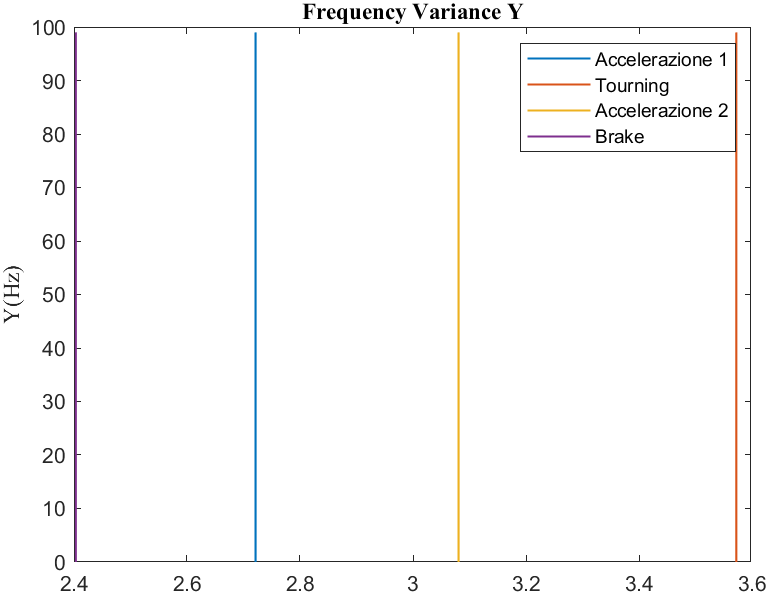
\includegraphics[height=.8\textheight]{figure/Vel/Trasformata/Frequency VarianceY}
%	\end{frame}
%	
%	\begin{frame}{{Frequency Variance Z}}
%		\centering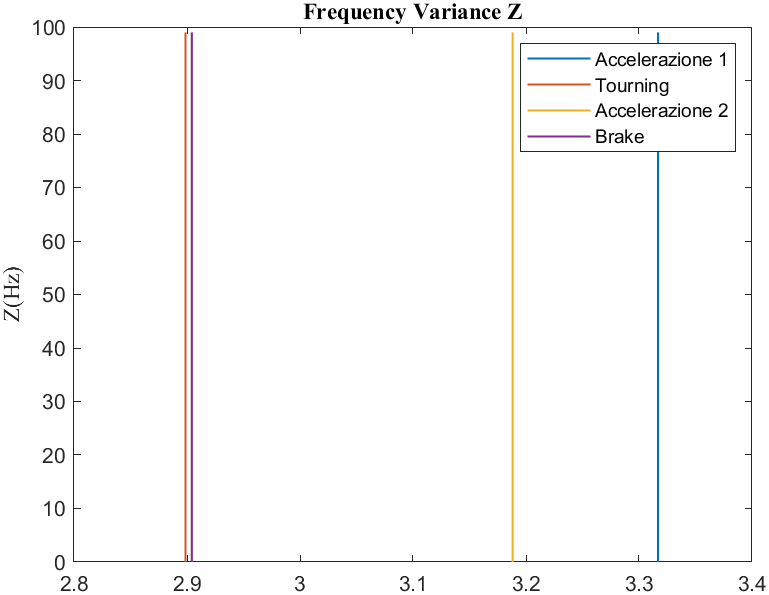
\includegraphics[height=.8\textheight]{figure/Vel/Trasformata/Frequency VarianceZ}
%	\end{frame}
%	
%	\begin{frame}
%		\color{blue}\centering\huge{\textbf{Spettro Velocità}}
%	\end{frame}
%	
%	\begin{frame}{{Spettro Accelerazione 1}}
%		\centering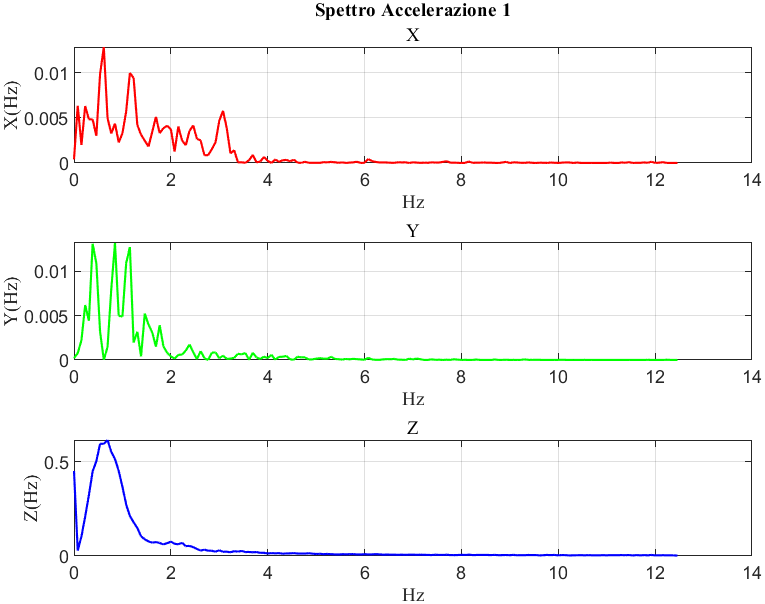
\includegraphics[height=.8\textheight]{figure/Vel/Trasformata/Spettro Accelerazione 1}
%	\end{frame}
%	
%	\begin{frame}{{Spettro Tourning}}
%		\centering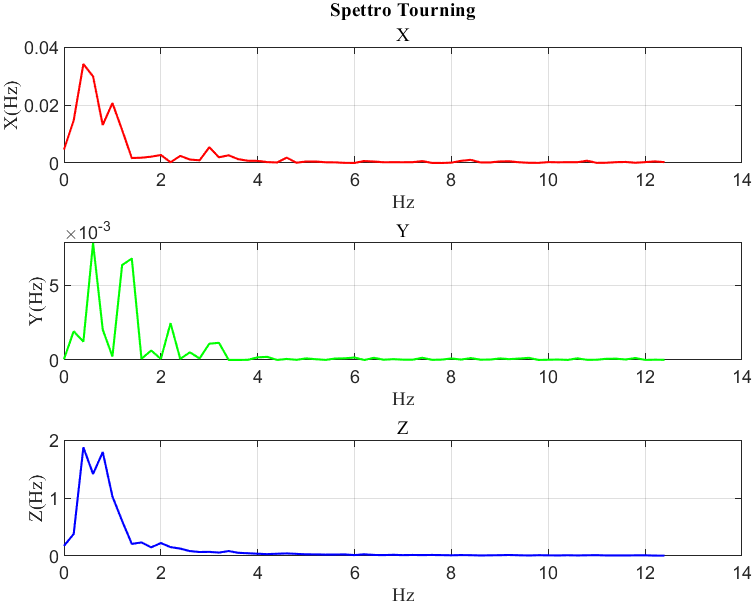
\includegraphics[height=.8\textheight]{figure/Vel/Trasformata/Spettro Tourning}
%	\end{frame}
%	
%	\begin{frame}{{Spettro Accelerazione 2}}
%		\centering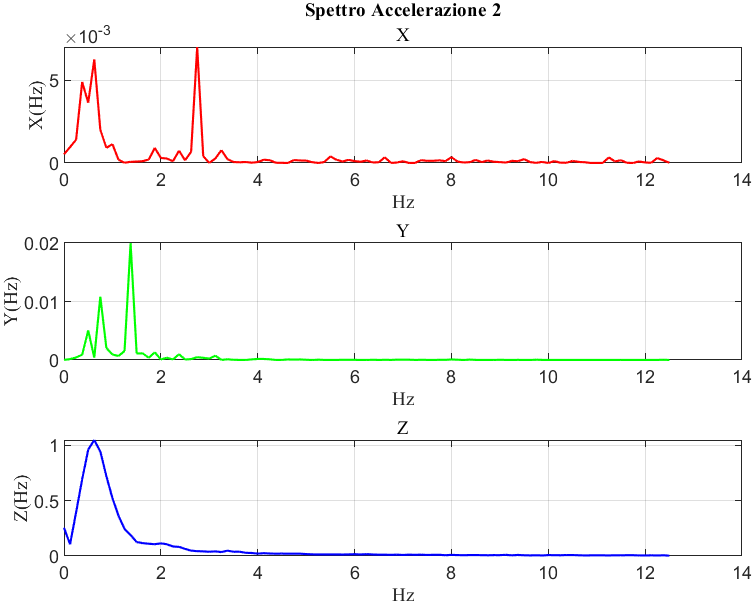
\includegraphics[height=.8\textheight]{figure/Vel/Trasformata/Spettro Accelerazione 2}
%	\end{frame}
%	
%	\begin{frame}{{Spettro Brake}}
%		\centering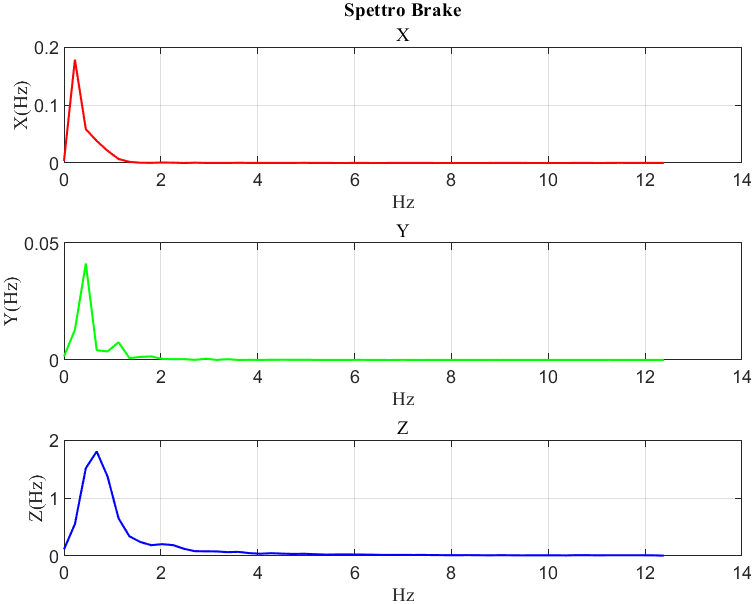
\includegraphics[height=.8\textheight]{figure/Vel/Trasformata/Spettro Brake}
%	\end{frame}
%	
%	\begin{frame}{{Spectral Entropy X}}
%		\centering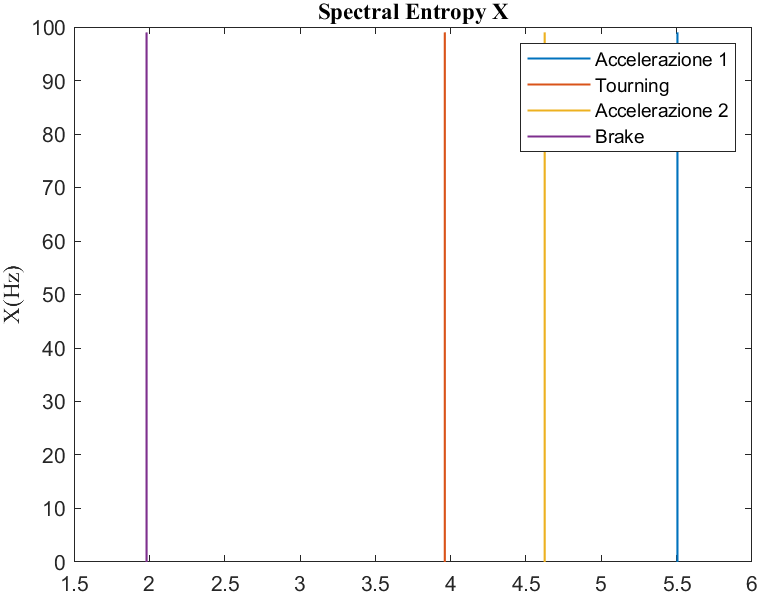
\includegraphics[height=.8\textheight]{figure/Vel/Trasformata/Spectral EntropyX}
%	\end{frame}
%	
%	\begin{frame}{{Spectral Entropy Y}}
%		\centering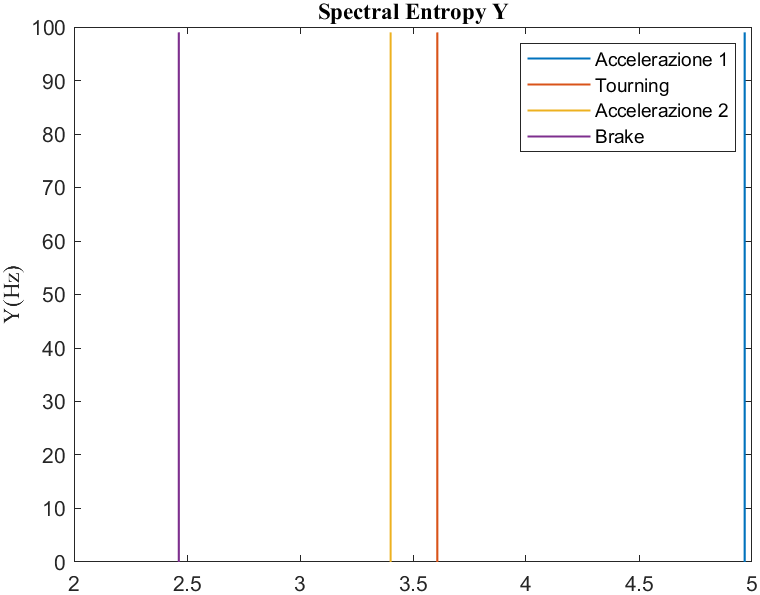
\includegraphics[height=.8\textheight]{figure/Vel/Trasformata/Spectral EntropyY}
%	\end{frame}
%	
%	\begin{frame}{{Spectral Entropy Z}}
%		\centering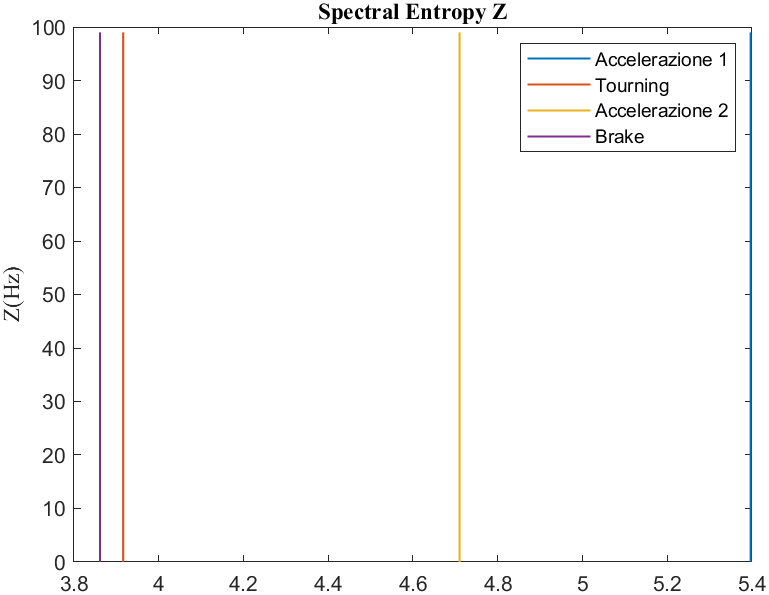
\includegraphics[height=.8\textheight]{figure/Vel/Trasformata/Spectral EntropyZ}
%	\end{frame}
	
\end{document}